\chapter{Methodology}\label{sec:3}

\begin{quote}
\textbf{DRAFT --- not submission-ready.} Citation venues were checked on
2026-10-11 (reference table in Chapter~\ref{sec:2}). Every number and
code detail in this chapter is traced to the writer brief,
\texttt{configs/\allowbreak{}}, \texttt{logs/\allowbreak{}}, or source
code (see the provenance table at the end).
\end{quote}

This chapter describes how the search agent is built, trained, and
evaluated. Section~\ref{sec:3.1} gives an overview of the research
design. Sections 3.2--3.6 describe the data, the search environment, the
proposed reward (VEGR), the policy model, and the training algorithm.
Section~\ref{sec:3.7} defines the evaluation protocol,
Section~\ref{sec:3.8} lists the experiments, and Section~\ref{sec:3.9}
reports the implementation and compute details.

\section{Research design overview}\label{sec:3.1}

The study is a controlled experiment. Only the reward function (and, in
two variants, the optimizer) changes between runs. The model, data,
environment, hyperparameters, and evaluation protocol stay fixed. This
lets differences in behaviour be attributed to the reward rather than to
other changes.

Each training episode follows the same loop (Figure~\ref{fig:3.1}):

\begin{enumerate}
\def\labelenumi{\arabic{enumi}.}
\tightlist
\item
  The agent receives a HotpotQA question.
\item
  It emits one action per turn: either \texttt{SEARCH{[}query{]}} or a
  terminal
  \texttt{ANSWER{[}.\allowbreak{}.\allowbreak{}.\allowbreak{}{]} CITATIONS{[}.\allowbreak{}.\allowbreak{}.\allowbreak{}{]}}.
\item
  The environment runs the search with BM25 over the question's own
  paragraphs and returns the results, or validates the answer and
  citations.
\item
  When the episode ends, the reward function scores it against
  HotpotQA's gold answer and gold supporting facts.
\item
  GRPO compares the rewards of 8 episodes on the same question and
  updates the LoRA adapter.
\end{enumerate}

\begin{figure}
\centering
\pandocbounded{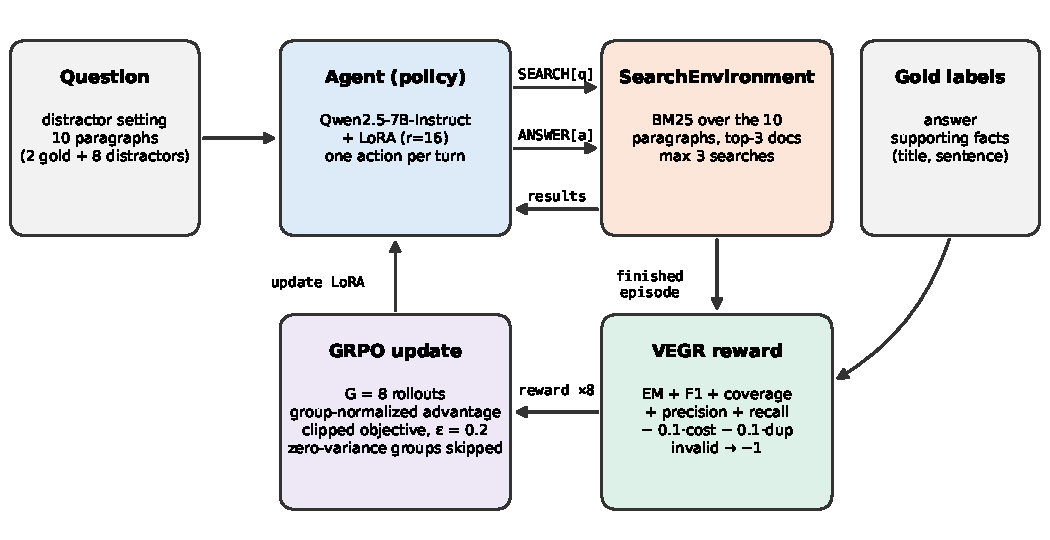
\includegraphics[keepaspectratio]{figures/fig3_1_system.pdf}}
\caption{One training step:}\label{fig:3.1}
\end{figure}

\begin{enumerate}
\def\labelenumi{\arabic{enumi}.}
\tightlist
\item
  The agent receives a HotpotQA question and takes up to 3
  \texttt{SEARCH} actions over the question's 10 paragraphs.
\item
  It ends with \texttt{ANSWER{[}a{]} CITATIONS{[}title|index; …{]}}.
\item
  The finished episode is scored by VEGR against the gold answer and
  supporting facts.
\item
  GRPO compares the rewards of 8 such episodes on the same question and
  updates the LoRA adapter.
\end{enumerate}

Drawn by
\texttt{scripts/\allowbreak{}make\_\allowbreak{}thesis\_\allowbreak{}figures.\allowbreak{}py}.

Three research questions guide the design (Chapter~\ref{sec:1}):

\begin{itemize}
\tightlist
\item
  \textbf{RQ1}: Does GRPO improve a 7B search agent over the un-tuned
  model?
\item
  \textbf{RQ2}: Does VEGR prevent the shortcut behaviour of answer-only
  reward, without losing accuracy?
\item
  \textbf{RQ3}: How do reward variants and optimizer fixes affect
  grounding and search behaviour?
\end{itemize}

\section{Dataset and splits}\label{sec:3.2}

The study uses \textbf{HotpotQA} (Yang et al., 2018), version 1.1, in
the \emph{distractor} setting. Each question comes with 10 Wikipedia
paragraphs: 2 gold paragraphs that contain the answer evidence, and 8
distractors. Each question is also annotated with \textbf{supporting
facts}, the (title, sentence index) pairs needed to answer it. These
annotations are what make a judge-free evidence reward possible: whether
a citation is correct can be checked by rule.

Rows that fail validation are skipped and logged with a reason (for
example, an empty sentence or a supporting-fact index out of range).

\textbf{Splits.} The split is produced by
\texttt{scripts/\allowbreak{}prepare\_\allowbreak{}splits.\allowbreak{}py}
and recorded in
\texttt{configs/\allowbreak{}evaluation/\allowbreak{}splits.\allowbreak{}json},
together with SHA-256 hashes of the source files.

\begin{itemize}
\tightlist
\item
  \textbf{Train / validation.} These are both drawn from the HotpotQA
  training file using a deterministic hash. Each question ID is mapped
  to a bucket in {[}0, 1) by taking the first 8 bytes of
  \texttt{sha256("7:" + question\_\allowbreak{}id)}. A question goes to
  train if the bucket is below 0.95, and to validation otherwise. This
  gives \textbf{85,573 training} and \textbf{4,452 validation}
  questions. The split does not depend on file order and can be
  reproduced exactly.
\item
  \textbf{Holdout.} The holdout is a frozen set of \textbf{300
  questions}: the first 300 valid rows of the HotpotQA dev file, stored
  in
  \texttt{configs/\allowbreak{}evaluation/\allowbreak{}holdout\_\allowbreak{}v1\_\allowbreak{}ids.\allowbreak{}json}
  along with a hash of the manifest. The holdout was never used to
  choose settings. All settings were chosen on the validation split, and
  the holdout is used only for the final numbers reported in
  Chapter~\ref{sec:4}.
\end{itemize}

\textbf{Training sample.} Each training run draws \textbf{256 questions}
from the training split. The sample depends on the run seed, so
different seeds see different questions (Section~\ref{sec:3.6}).

\section{Search environment}\label{sec:3.3}

The environment (\texttt{SearchEnvironment},
\texttt{src/\allowbreak{}needle/\allowbreak{}environment/\allowbreak{}search.\allowbreak{}py})
is a bounded, resettable search session over a single question.

\textbf{Corpus and retriever.} The searchable corpus is the question's
own 10 paragraphs. Retrieval uses Okapi BM25 (Robertson \& Zaragoza,
2009), via the \texttt{rank\_\allowbreak{}bm25} implementation with its
default parameters. Each paragraph is indexed as its title plus all its
sentences, tokenized into case-folded Unicode word tokens. A search
returns the \textbf{top 3} documents. Ties are broken by original
document order, so retrieval is deterministic. Each returned document is
shown in full, with numbered sentences.

\textbf{Budget.} An episode allows at most \textbf{3 searches}.

\textbf{Action grammar.} On each turn the agent must output exactly one
action:

\begin{itemize}
\tightlist
\item
  \texttt{SEARCH{[}query{]}} runs a BM25 search and spends one unit of
  budget.
\item
  \texttt{ANSWER{[}answer{]} CITATIONS{[}title|index; title|index; .\allowbreak{}.\allowbreak{}.\allowbreak{}{]}}
  gives the final answer together with the cited evidence sentences.
  This action ends the episode.
\end{itemize}

\textbf{Validation and failure types.} An episode is \textbf{invalid} if
any of the following happens:

\begin{itemize}
\tightlist
\item
  \emph{Protocol failure}: the output does not match the grammar (for
  example, extra text, or citations attached to a SEARCH action).
\item
  \emph{Evidence failure}: a citation refers to a title or sentence
  index that never appeared in any search result in the episode. In
  practice this mostly means invented citations.
\item
  \emph{Budget failure}: the agent uses all its searches and still does
  not answer.
\end{itemize}

Invalid episodes receive the protocol penalty of −1 during training
(Section~\ref{sec:3.4}) and count as wrong during evaluation
(Section~\ref{sec:3.7}).

\textbf{Known loophole.} An answer with an empty citation list
(\texttt{ANSWER{[}x{]}} or \texttt{ANSWER{[}x{]} CITATIONS{[}{]}}) is
accepted as valid. The prompt itself allows \texttt{CITATIONS{[}{]}} for
the case where no citation can be validated. We did not close this
loophole, so that every run is trained and evaluated in the same
environment. Chapter~\ref{sec:4} reports how the answer-only reward
exploited it.

\section{Proposed reward: VEGR}\label{sec:3.4}

The \textbf{Verifiable Evidence-Grounded Reward (VEGR)} is implemented
in
\texttt{src/\allowbreak{}needle/\allowbreak{}rewards/\allowbreak{}\_\allowbreak{}\_\allowbreak{}init\_\allowbreak{}\_\allowbreak{}.\allowbreak{}py}.
Every term is computed by rule from HotpotQA's gold annotations, so no
LLM judge is involved.

Let \emph{G} be the set of gold supporting facts (title, sentence index)
and \emph{C} the set of sentences the agent cites. For a valid episode:

\[
R_{\text{VEGR}} = \text{EM} + \text{F1} + \text{Cov} + \text{Prec} + \text{RetR} - 0.1\cdot\text{Cost} - 0.1\cdot\text{Dup}
\]

{\def\LTcaptype{none} % do not increment counter
\begin{longtable}[]{@{}
  >{\raggedright\arraybackslash}p{(\linewidth - 4\tabcolsep) * \real{0.3333}}
  >{\raggedright\arraybackslash}p{(\linewidth - 4\tabcolsep) * \real{0.3333}}
  >{\raggedright\arraybackslash}p{(\linewidth - 4\tabcolsep) * \real{0.3333}}@{}}
\toprule\noalign{}
\begin{minipage}[b]{\linewidth}\raggedright
Term
\end{minipage} & \begin{minipage}[b]{\linewidth}\raggedright
Definition
\end{minipage} & \begin{minipage}[b]{\linewidth}\raggedright
Range
\end{minipage} \\
\midrule\noalign{}
\endhead
\bottomrule\noalign{}
\endlastfoot
EM & normalized exact match between predicted and gold answer & \{0,
1\} \\
F1 & token-level F1 between predicted and gold answer & {[}0, 1{]} \\
Cov (evidence coverage) & \textbar G ∩ C\textbar{} /
\textbar G\textbar{} & {[}0, 1{]} \\
Prec (citation precision) & \textbar G ∩ C\textbar{} /
\textbar C\textbar, defined as 0 when C is empty & {[}0, 1{]} \\
RetR (retrieval recall) & fraction of gold documents that appeared in
any search result & {[}0, 1{]} \\
Cost (search cost) & searches used / budget (3) & {[}0, 1{]} \\
Dup (duplicate-query penalty) & (number of queries − number of unique
queries) / number of queries & {[}0, 1) \\
\end{longtable}
}

An \textbf{invalid} episode receives \textbf{R = −1}, regardless of the
other terms. This protocol penalty is what makes VEGR enforce the action
grammar. Because an invented citation is an evidence failure, the agent
cannot raise its precision by citing sentences it never retrieved.

The terms fall into three groups, each aimed at a different failure:

\begin{itemize}
\tightlist
\item
  \textbf{Answer terms (EM, F1)} reward correctness. F1 gives partial
  credit, so the reward is less sparse than EM alone.
\item
  \textbf{Evidence terms (Cov, Prec)} reward citing the right sentences.
  Precision alone could be satisfied by citing a single safe sentence,
  and coverage alone by citing everything, so both are included
  (cf.~ALCE; Gao et al., 2023).
\item
  \textbf{Search terms (RetR, Cost, Dup)} reward finding the gold
  documents and penalize wasted or repeated searches. The penalties have
  a small weight (0.1) so that they shape search behaviour without
  discouraging search altogether.
\end{itemize}

The individual terms are not new. The contribution is combining them
into a judge-free reward for multi-turn search agents, together with a
controlled evaluation of what the combination changes
(Section~\ref{sec:3.8}). All weights are untuned defaults. This is a
limitation, discussed in Chapter~\ref{sec:5}.

\textbf{Worked example.} Table~\ref{tbl:3.1} scores two real holdout
episodes for the same question (\texttt{5abd94525542992ac4f382d2},
``Which company formed the boy group that debuted with \emph{2014
S/S}?''). Both answer ``YG Entertainment'' correctly. Under the
outcome-only reward (R0) both receive the same reward, 1. VEGR separates
them: one is fully grounded, the other has no evidence.

\begin{longtable}[]{@{}
  >{\raggedright\arraybackslash}p{(\linewidth - 4\tabcolsep) * \real{0.3333}}
  >{\raggedright\arraybackslash}p{(\linewidth - 4\tabcolsep) * \real{0.3333}}
  >{\raggedright\arraybackslash}p{(\linewidth - 4\tabcolsep) * \real{0.3333}}@{}}
\caption{VEGR terms for two correct answers to the same question. Values
are taken from
\texttt{results/\allowbreak{}2026-\allowbreak{}10-\allowbreak{}10-\allowbreak{}batch/\allowbreak{}\{r1\_\allowbreak{}full\_\allowbreak{}seed8,r0\_\allowbreak{}outcome\_\allowbreak{}seed8\}/\allowbreak{}episodes.\allowbreak{}jsonl}.}\label{tbl:3.1}\tabularnewline
\toprule\noalign{}
\begin{minipage}[b]{\linewidth}\raggedright
\end{minipage} & \begin{minipage}[b]{\linewidth}\raggedright
Episode A (R1 seed 8)
\end{minipage} & \begin{minipage}[b]{\linewidth}\raggedright
Episode B (R0 seed 8)
\end{minipage} \\
\midrule\noalign{}
\endfirsthead
\toprule\noalign{}
\begin{minipage}[b]{\linewidth}\raggedright
\end{minipage} & \begin{minipage}[b]{\linewidth}\raggedright
Episode A (R1 seed 8)
\end{minipage} & \begin{minipage}[b]{\linewidth}\raggedright
Episode B (R0 seed 8)
\end{minipage} \\
\midrule\noalign{}
\endhead
\bottomrule\noalign{}
\endlastfoot
Actions &
\texttt{SEARCH{[}S/\allowbreak{}S 2014 debut South Korean boy group{]}}
→ \texttt{SEARCH{[}WINNER YG Entertainment{]}} →
\texttt{ANSWER{[}YG Entertainment{]} CITATIONS{[}2014 S/\allowbreak{}S\textbackslash{}|0; Winner (band)\textbackslash{}|0{]}}
&
\texttt{SEARCH{[}2014 S/\allowbreak{}S debut album South Korean boy group formed by{]}}
→ \texttt{ANSWER{[}YG Entertainment{]}} \\
EM & 1 & 1 \\
F1 & 1 & 1 \\
Evidence coverage & 1 (both gold sentences cited) & 0 (nothing cited) \\
Citation precision & 1 & 0 \\
Retrieval recall & 1 (both gold documents retrieved) & 0.5 (one of
two) \\
− 0.1 · search cost & − 0.1 · 2/3 = − 0.067 & − 0.1 · 1/3 = − 0.033 \\
− 0.1 · duplicate penalty & 0 & 0 \\
\textbf{VEGR total} & \textbf{4.933} & \textbf{2.467} \\
Outcome-only reward (R0) & 1 & 1 \\
\end{longtable}

\textbf{Reward variants.} Three variants change one aspect of VEGR at a
time:

\begin{itemize}
\tightlist
\item
  \textbf{R0, outcome-only (baseline reward).} R = EM. All other weights
  are 0, but invalid episodes still receive −1. This mirrors
  outcome-reward search agents such as Search-R1 (Jin et al., 2025).
\item
  \textbf{R2, gated penalties.} This is VEGR, except that the
  search-cost and duplicate penalties apply only when EM = 1. The idea
  is to avoid penalizing search on questions the agent has not yet
  solved.
\item
  \textbf{R3, coverage ×2.} This is VEGR with the evidence-coverage
  weight raised from 1 to 2. It targets the ``precise but incomplete''
  citation pattern described in Chapter~\ref{sec:4}.
\end{itemize}

\section{Policy model}\label{sec:3.5}

\textbf{Base model.} The policy is \textbf{Qwen2.5-7B-Instruct} (Qwen
Team, 2024), loaded from local weights in bf16.

\textbf{Prompt.} The prompt is deterministic and built by
\texttt{build\_\allowbreak{}prompt} in
\texttt{src/\allowbreak{}needle/\allowbreak{}inference/\allowbreak{}runner.\allowbreak{}py}.
It is wrapped in the model's chat template. The prompt:

\begin{enumerate}
\def\labelenumi{\arabic{enumi}.}
\tightlist
\item
  Describes the role (``You are a careful evidence-seeking QA agent'').
\item
  States the action grammar, gives a worked example
  (\texttt{ANSWER{[}United States{]} CITATIONS{[}Ursula K.\allowbreak{} Le Guin|1; The Left Hand of Darkness|1{]}}),
  and lists formatting rules: one \texttt{title|index} per citation,
  semicolon-separated, no text after the closing bracket, titles copied
  exactly, never invent a title.
\item
  Gives the question and the remaining search budget.
\item
  Lists all search results so far. For each search, it shows the query
  and then every returned document as \texttt{{[}Title{]}} followed by
  \texttt{index: sentence} lines.
\end{enumerate}

The prompt is rebuilt from scratch every turn, so the model always sees
the full search history. Appendix A gives the complete prompt for one
real holdout question, at the point just before the agent gives its
final answer.

\textbf{Adapter.} Training uses LoRA (Hu et al., 2022) with rank r = 16,
α = 32, and dropout 0. The adapter is applied to all attention and MLP
projections (q, k, v, o, gate, up, down). The base weights stay frozen,
which makes training on a single 48 GB GPU possible.

\section{Training algorithm}\label{sec:3.6}

Training uses \textbf{Group Relative Policy Optimization} (GRPO; Shao et
al., 2024), extended to multi-turn episodes. The implementation is in
\texttt{scripts/\allowbreak{}train\_\allowbreak{}grpo.\allowbreak{}py}
and
\texttt{src/\allowbreak{}needle/\allowbreak{}training/\allowbreak{}grpo.\allowbreak{}py}.

\textbf{Rollouts.} For each training question, the current policy runs
\textbf{G = 8} full episodes, sampling with temperature 1.0 and top-p
1.0. Each action is limited to 128 new tokens. Each episode receives one
scalar reward from the reward function of the run (R0--R3).

\textbf{Advantage.} Each reward is normalized within its group:

\[
A_i = \frac{r_i - \operatorname{mean}(r_{1..G})}{\operatorname{std}(r_{1..G}) + 10^{-6}}
\]

All actions in an episode share the episode's advantage. If all 8
rewards in a group are equal, every advantage is zero and the group
carries no learning signal. Such \textbf{zero-variance groups are
skipped}: no update is made. The number of skipped steps is logged, and
it turns out to be an important diagnostic (Chapter~\ref{sec:4}).

\textbf{Objective.} The update uses the PPO-style clipped surrogate
(Schulman et al., 2017) with ε = 0.2. Each rollout's log-probability is
the \textbf{mean over all tokens the agent generated in that episode},
across all its actions. Prompt and observation tokens are excluded. The
ratio ρ is therefore computed once per rollout.

\[
\mathcal{L} = -\,\mathbb{E}\left[\min\left(\rho\,A,\; \operatorname{clip}(\rho,\,1-\varepsilon,\,1+\varepsilon)\,A\right)\right],
\qquad \rho = \exp\left(\log\pi_\theta - \log\pi_{\theta_\text{old}}\right)
\]

There is \textbf{no KL penalty} to a reference model. Invalid rollouts
stay in the batch, so the −1 penalty actively pushes the policy away
from malformed actions.

\textbf{Optimization.} AdamW with learning rate 2 × 10⁻⁵, gradient-norm
clipping at 1.0, bf16, and gradient checkpointing. A run makes one pass
over its 256 questions (256 steps, one question per step).

\textbf{Seeds.} Runs use seeds 7, 8, and 9. A seed fixes both the
256-question training sample and the random state used for sampling
rollouts. Seed-to-seed differences therefore reflect both data and
optimization noise.

\textbf{Optimizer variants.} Two variants change the optimizer instead
of the reward:

\begin{itemize}
\tightlist
\item
  \textbf{Dr.~GRPO advantages} (Liu et al., 2025), used in R4. The
  advantage is computed without dividing by the standard deviation, A\_i
  = r\_i − mean(r). This removes the scaling that amplifies groups whose
  rewards are nearly equal.
\item
  \textbf{DAPO-style dynamic sampling} (Yu et al., 2025), used in
  R0-dyn. Zero-variance groups do not count toward the step budget. The
  trainer keeps drawing questions, from a pool of up to 512, until it
  has made 256 actual optimizer updates. This tests whether R0's
  shortcut comes from having too few informative updates.
\end{itemize}

\textbf{Pseudocode.}

\begin{Verbatim}
for step, question in enumerate(sample(train_split, 256, seed)):
    episodes = [run_episode(policy, question) for _ in range(8)]   # multi-turn
    rewards  = [reward_fn(ep, gold(question)) for ep in episodes]  # VEGR or variant; invalid → −1
    if all rewards equal:
        log_skip(step); continue                                    # zero-variance group
    A = (rewards − mean(rewards)) / (std(rewards) + 1e-6)          # Dr. GRPO: no division
    for each episode i:
        ρ = exp(mean_token_logp_θ(actions_i) − mean_token_logp_old(actions_i))  # mean over all action tokens
        loss += −min(ρ·A_i, clip(ρ, 0.8, 1.2)·A_i)
    update LoRA with AdamW (lr 2e-5, grad clip 1.0)
\end{Verbatim}

\section{Evaluation protocol}\label{sec:3.7}

\textbf{Setting.} Every model is evaluated on the same frozen
\textbf{300-question holdout}, with greedy decoding and \textbf{no
retries}. If an action is malformed, the episode fails.

\textbf{Metrics.}

\begin{itemize}
\tightlist
\item
  \textbf{EM (all)} is the headline accuracy number. Every invalid
  episode counts as 0, so the denominator is always 300.
\item
  \textbf{Completed episodes} is the number of valid episodes out of
  300. Failures are broken down by type (evidence, protocol, budget).
\item
  \textbf{Quality metrics} are F1, evidence coverage, citation
  precision, retrieval recall, and searches per episode. Each is
  averaged over completed episodes only, using the definitions in
  Section~\ref{sec:3.4}.
\item
  \textbf{Grounded EM} counts an episode only if EM = 1, it has at least
  one citation, and every citation is a gold supporting fact. This is a
  strict metric: a correct answer with one non-gold citation does not
  count. It is the measure most directly tied to the thesis claim that
  answers should be correct \emph{and} supported by evidence.
\item
  \textbf{Behavioural diagnostics} come from the episode and training
  logs. They include the share of episodes that repeat a query, the
  distribution of citation counts and cited sentence indices, the
  invalid rate during training, and the number of skipped
  (zero-variance) training steps.
\end{itemize}

\textbf{Statistics.} Following Agarwal et al.~(2021) and Henderson et
al.~(2018), single runs are not treated as conclusive.

\begin{itemize}
\tightlist
\item
  Differences in EM between two models are tested with a \textbf{paired
  bootstrap} over the 300 holdout questions: 10,000 resamples and a 95\%
  percentile confidence interval. A difference is called significant
  only if the CI excludes 0.
\item
  Each reward variant is trained with \textbf{3 seeds} (7, 8, 9).
  Results are reported per seed and as the mean across seeds.
\item
  Since seeds of the same method can differ by several EM points, a
  method difference is only claimed when it holds across seeds, not when
  it shows up for a single seed.
\end{itemize}

\section{Experiment matrix}\label{sec:3.8}

{\def\LTcaptype{none} % do not increment counter
\begin{longtable}[]{@{}
  >{\raggedright\arraybackslash}p{(\linewidth - 8\tabcolsep) * \real{0.2000}}
  >{\raggedright\arraybackslash}p{(\linewidth - 8\tabcolsep) * \real{0.2000}}
  >{\raggedright\arraybackslash}p{(\linewidth - 8\tabcolsep) * \real{0.2000}}
  >{\raggedright\arraybackslash}p{(\linewidth - 8\tabcolsep) * \real{0.2000}}
  >{\raggedright\arraybackslash}p{(\linewidth - 8\tabcolsep) * \real{0.2000}}@{}}
\toprule\noalign{}
\begin{minipage}[b]{\linewidth}\raggedright
ID
\end{minipage} & \begin{minipage}[b]{\linewidth}\raggedright
Name
\end{minipage} & \begin{minipage}[b]{\linewidth}\raggedright
Reward
\end{minipage} & \begin{minipage}[b]{\linewidth}\raggedright
Optimizer
\end{minipage} & \begin{minipage}[b]{\linewidth}\raggedright
Seeds
\end{minipage} \\
\midrule\noalign{}
\endhead
\bottomrule\noalign{}
\endlastfoot
B0 & Un-tuned baseline & --- (no training) & --- & --- \\
R0 & Outcome-only & EM, invalid −1 & GRPO & 7, 8, 9 \\
R1 & \textbf{VEGR} & full VEGR & GRPO & 7, 8, 9 \\
R2 & Gated & VEGR, penalties only when EM = 1 & GRPO & 7, 8, 9 \\
R3 & Coverage ×2 & VEGR, coverage weight 2 & GRPO & 7, 8, 9 \\
R4 & VEGR + Dr.~GRPO & full VEGR & GRPO, no std division & 7, 8, 9 \\
R0-dyn & Outcome-only + dynamic sampling & EM, invalid −1 & GRPO + DAPO
dynamic sampling & 8 \\
\end{longtable}
}

The comparisons map onto the research questions:

\begin{itemize}
\tightlist
\item
  \textbf{RQ1:} every trained run against B0.
\item
  \textbf{RQ2:} R1 against R0. Same optimizer, same seeds, different
  reward.
\item
  \textbf{RQ3:}

  \begin{itemize}
  \tightlist
  \item
    R2 and R3 against R1 test reward design.
  \item
    R4 against R1, and R0-dyn against R0, test optimizer fixes.
  \item
    R0-dyn is the key control. If dynamic sampling alone removes R0's
    shortcut, the problem was the optimizer and not the reward. If it
    does not, the evidence reward is necessary.
  \end{itemize}
\end{itemize}

R0-dyn was run on a single seed (seed 8) as a \textbf{diagnostic
experiment}, not as one of the main methods.

\begin{itemize}
\tightlist
\item
  \textbf{Why one seed (cost).} Dynamic sampling discards zero-variance
  groups, and R0 seed 8 skipped 128 of its 256 steps. Reaching 256 real
  updates is therefore expected to take up to about 512 questions,
  roughly twice the rollouts and cost of a standard run. The budget
  extension originally planned this test on two seeds. It was cut to one
  so that the 3-seed runs of the main methods (R0--R4) fit the budget.
  {[}TODO: replace ``expected'' with the actual number of questions
  drawn and the run time.{]}
\item
  \textbf{Why seed 8.} It is the seed on which outcome-only training
  collapsed to uncited answers. The question is narrow: does an
  optimizer-level fix alone prevent this shortcut where it actually
  happened? A seed on which R0 did not collapse could not answer that.
\item
  \textbf{How it is read.} R0-dyn is interpreted as a case study about
  mechanism, not as a statistically supported comparison between
  methods.
\end{itemize}

\textbf{Planned vs.~post hoc.} B0, R0, R1, and R2 were specified before
the multi-seed batch ran
(\texttt{logs/\allowbreak{}2026-\allowbreak{}10-\allowbreak{}10-\allowbreak{}r0-\allowbreak{}r1-\allowbreak{}r2-\allowbreak{}batch.\allowbreak{}md}).
Only the single R1 seed-7 run existed at that point. R3, R4, and R0-dyn
were added on 2026-10-11, after the R0/R1/R2 results had been analysed
(\texttt{docs/\allowbreak{}research/\allowbreak{}2026-\allowbreak{}10-\allowbreak{}11-\allowbreak{}results-\allowbreak{}diagnosis-\allowbreak{}and-\allowbreak{}improvements.\allowbreak{}md}).
They respond to specific observations: low evidence coverage, and R0's
skipped steps and shortcuts. They are therefore \textbf{exploratory
follow-ups}, and Chapter~\ref{sec:4} reports them as such rather than as
confirmatory tests.

\section{Implementation and compute}\label{sec:3.9}

\textbf{Software.} Python 3.11 (managed with \texttt{uv}), Transformers
4.57.6, PEFT 0.21.2, and \texttt{rank\_\allowbreak{}bm25}. PyTorch
differs between runs:

\begin{itemize}
\tightlist
\item
  The first runs (B0 and R1 seed 7) used \textbf{2.14.1+cu130}.
\item
  All later runs used \textbf{2.11.0+cu128}, because the later pod's GPU
  driver supported only CUDA 12.8.
\end{itemize}

This is reported as a limitation when comparing against R1 seed 7.
Training and evaluation run offline from local weights, with Hugging
Face offline mode on.

\textbf{Hardware and cost.} One NVIDIA L40S (48 GB) on RunPod at about
\$1.10 per hour. One run (training plus holdout evaluation) takes about
2.05 hours, or roughly \textbf{\$2.25}. The total project budget is
about \$45. \texttt{{[}TODO: final cost table after the fixes batch{]}}

\textbf{Reproducibility.}

\begin{itemize}
\tightlist
\item
  Splits are fixed by hashed manifests (Section~\ref{sec:3.2}).
\item
  Every run is defined by a JSON config in
  \texttt{configs/\allowbreak{}training/\allowbreak{}} and writes
  \texttt{run\_\allowbreak{}metadata.\allowbreak{}json} (library
  versions, seed, config), \texttt{summary.\allowbreak{}json},
  \texttt{episodes.\allowbreak{}jsonl} (every evaluation episode), and
  \texttt{metrics.\allowbreak{}jsonl} (per-step training metrics) to
  \texttt{results/\allowbreak{}<date>/\allowbreak{}<run>/\allowbreak{}}.
\item
  Each batch has a dated log in \texttt{logs/\allowbreak{}}.
\item
  The step-by-step procedure for reproducing the runs on RunPod is in
  \texttt{docs/\allowbreak{}runbooks/\allowbreak{}runpod.\allowbreak{}md}.
\end{itemize}

\begin{center}\rule{0.5\linewidth}{0.5pt}\end{center}

\section{Provenance (remove before
submission)}\label{provenance-remove-before-submission}

{\def\LTcaptype{none} % do not increment counter
\begin{longtable}[]{@{}
  >{\raggedright\arraybackslash}p{(\linewidth - 2\tabcolsep) * \real{0.5000}}
  >{\raggedright\arraybackslash}p{(\linewidth - 2\tabcolsep) * \real{0.5000}}@{}}
\toprule\noalign{}
\begin{minipage}[b]{\linewidth}\raggedright
Claim in this chapter
\end{minipage} & \begin{minipage}[b]{\linewidth}\raggedright
Source
\end{minipage} \\
\midrule\noalign{}
\endhead
\bottomrule\noalign{}
\endlastfoot
Split algorithm, 0.95 fraction, 85,573 / 4,452 counts, holdout = first
300 valid dev rows &
\texttt{configs/\allowbreak{}evaluation/\allowbreak{}splits.\allowbreak{}json},
\texttt{scripts/\allowbreak{}prepare\_\allowbreak{}splits.\allowbreak{}py} \\
BM25 (\texttt{rank\_\allowbreak{}bm25.\allowbreak{}BM25Okapi},
defaults), tokenizer, tie-breaking &
\texttt{src/\allowbreak{}needle/\allowbreak{}retrieval/\allowbreak{}bm25.\allowbreak{}py} \\
Top-k 3, budget 3, failure types, no-citation loophole & writer brief
§3;
\texttt{src/\allowbreak{}needle/\allowbreak{}environment/\allowbreak{}search.\allowbreak{}py} \\
Prompt content, chat template &
\texttt{src/\allowbreak{}needle/\allowbreak{}inference/\allowbreak{}runner.\allowbreak{}py::build\_\allowbreak{}prompt};
\texttt{src/\allowbreak{}needle/\allowbreak{}training/\allowbreak{}local\_\allowbreak{}policy.\allowbreak{}py} \\
Reward formula and weights &
\texttt{src/\allowbreak{}needle/\allowbreak{}rewards/\allowbreak{}\_\allowbreak{}\_\allowbreak{}init\_\allowbreak{}\_\allowbreak{}.\allowbreak{}py};
writer brief §3 \\
GRPO settings, per-rollout sequence-mean ratio, clipping &
\texttt{src/\allowbreak{}needle/\allowbreak{}training/\allowbreak{}grpo.\allowbreak{}py},
\texttt{scripts/\allowbreak{}train\_\allowbreak{}grpo.\allowbreak{}py} \\
Dynamic sampling (512 pool, 256 updates) &
\texttt{logs/\allowbreak{}2026-\allowbreak{}10-\allowbreak{}11-\allowbreak{}fixes-\allowbreak{}batch.\allowbreak{}md} \\
Library versions, torch change and reason &
\texttt{results/\allowbreak{}*/\allowbreak{}run\_\allowbreak{}metadata.\allowbreak{}json};
\texttt{logs/\allowbreak{}2026-\allowbreak{}10-\allowbreak{}10-\allowbreak{}r0-\allowbreak{}r1-\allowbreak{}r2-\allowbreak{}batch.\allowbreak{}md} \\
Cost per run, budget & writer brief §3;
\texttt{logs/\allowbreak{}2026-\allowbreak{}10-\allowbreak{}11-\allowbreak{}fixes-\allowbreak{}batch.\allowbreak{}md} \\
\texttt{uv} & \texttt{uv.\allowbreak{}lock} in repo root \\
\end{longtable}
}
